\documentclass[aspectratio=169,11pt]{beamer}

\def\courseTitle{Industrial Security (Master)}
\def\courseSubtitle{Section 03 -- Advanced Industrial Protocols}
\def\sectionNumber{03}
\def\sectionTitle{Advanced Industrial Protocols}

% =====================================================================
% Industrial Security lecture series -- modern Beamer preamble.
%
% Each slide deck must define the following BEFORE \input{}-ing this:
%   \def\courseTitle{...}        e.g. Industrial Security (Bachelor)
%   \def\courseSubtitle{...}     e.g. Section 3 -- Network Architecture
%   \def\sectionNumber{...}      e.g. 03
%   \def\sectionTitle{...}       e.g. Industrial Network Architectures
%
% Optional:
%   \def\courseAuthor{...}       defaults to "Lecture Notes"
%   \def\courseInstitute{...}    defaults to "Department of Computer Science"
%   \def\companyLogo{...}        path to a logo image (PDF/PNG/JPG).
%
% Callout macros (use anywhere inside a frame):
%   \begin{notebox}{title}      ... \end{notebox}
%   \begin{importantbox}{title} ... \end{importantbox}
%   \begin{warningbox}{title}   ... \end{warningbox}
%   \begin{tipbox}{title}       ... \end{tipbox}
%   \begin{defbox}{title}       ... \end{defbox}
%   \begin{takeawaybox}{title}  ... \end{takeawaybox}
%   \begin{quotebox}            ... \end{quotebox}
% =====================================================================

% --- Speaker-notes mode (toggled by Makefile via -usepretex) ----------
% When notesmode=1, build a side-by-side slide+notes PDF for the
% lecturer. When unset/0, build the clean slides-only PDF.
\providecommand{\notesmode}{0}
\ifnum\notesmode=1
  \usepackage{pgfpages}
  \setbeameroption{show notes on second screen=right}
  \setbeamerfont{note page}{size=\small}
\fi

\usepackage[utf8]{inputenc}
\usepackage[T1]{fontenc}
\usepackage[english]{babel}
% Modern type pair: IBM Plex Sans for text, IBM Plex Mono for code.
% Math stays in lmodern; Plex is the dominant family on every text frame.
\usepackage{plex-sans}
\usepackage{plex-mono}
\renewcommand{\familydefault}{\sfdefault}
\usepackage[activate={true,nocompatibility},final,tracking=true,kerning=true,spacing=true,factor=1100,stretch=10,shrink=10]{microtype}
\usepackage{graphicx}
\usepackage{listings}
\usepackage{xcolor}
\usepackage{colortbl}
\usepackage{tikz}
\usepackage{booktabs}
\usepackage{array}
\usepackage{hyperref}
\usepackage{amsmath}
\usepackage{amssymb}
\usepackage{tcolorbox}
\tcbuselibrary{skins, breakable, raster}
\usepackage{fontawesome5}

% =====================================================================
% Shared TikZ styles for the Industrial Security lecture series.
% Loaded by every slide deck and exercise sheet that uses TikZ.
% =====================================================================

\usetikzlibrary{
  arrows.meta,
  shapes,
  shapes.geometric,
  shapes.symbols,
  shapes.multipart,
  positioning,
  fit,
  calc,
  backgrounds,
  decorations.pathmorphing,
  decorations.pathreplacing,
  decorations.text,
  patterns,
  matrix,
  shadows
}

% --- colour palette --------------------------------------------------
\definecolor{isOT}{HTML}{1F4E79}     % OT (deep blue)
\definecolor{isIT}{HTML}{6F2DA8}     % IT (purple)
\definecolor{isSafety}{HTML}{C00000} % safety red
\definecolor{isNet}{HTML}{2E7D32}    % network green
\definecolor{isAttack}{HTML}{B23A48} % attack red
\definecolor{isAccent}{HTML}{E08E0B} % amber
\definecolor{isMute}{HTML}{6B6B6B}   % grey
\definecolor{isLight}{HTML}{EDF2F8}  % light background
\definecolor{isPLC}{HTML}{2C5282}
\definecolor{isHMI}{HTML}{2F855A}
\definecolor{isSCADA}{HTML}{6B46C1}

% --- generic node styles --------------------------------------------
\tikzset{
  isnode/.style={
    draw, rounded corners=2pt, minimum height=8mm, minimum width=18mm,
    font=\small, align=center, thick
  },
  isbox/.style={isnode, fill=isLight},
  plc/.style={isnode, fill=isPLC!15, draw=isPLC, thick},
  hmi/.style={isnode, fill=isHMI!15, draw=isHMI, thick},
  scada/.style={isnode, fill=isSCADA!15, draw=isSCADA, thick},
  sensor/.style={isnode, fill=isNet!10, draw=isNet, minimum height=6mm, minimum width=14mm, font=\scriptsize},
  actuator/.style={isnode, fill=isAccent!15, draw=isAccent, minimum height=6mm, minimum width=14mm, font=\scriptsize},
  firewall/.style={isnode, fill=isAttack!15, draw=isAttack, thick},
  server/.style={isnode, fill=isMute!15, draw=isMute!80, thick},
  switch/.style={isnode, fill=isLight, draw=black!60, minimum height=6mm, minimum width=14mm, font=\scriptsize},
  workstation/.style={isnode, fill=white, draw=isOT, thick},
  attacker/.style={isnode, fill=isAttack!20, draw=isAttack, thick, font=\small\bfseries},
  inetnode/.style={draw, ellipse, minimum width=24mm, minimum height=10mm, font=\scriptsize, fill=isLight, thick},
  process/.style={isnode, fill=isOT!15, draw=isOT, thick, minimum width=24mm},
  zone/.style={
    draw, rounded corners=4pt, thick, dashed, inner sep=4mm
  },
  conduit/.style={-{Stealth[length=2.5mm]}, thick, isNet!80!black},
  attack/.style={-{Stealth[length=2.5mm]}, thick, isAttack, dashed},
  flow/.style={-{Stealth[length=2.5mm]}, thick, isOT!70!black},
  netline/.style={thick, black!60},
  axisline/.style={-{Stealth[length=2mm]}, thick, black!70},
  tag/.style={font=\scriptsize\itshape, fill=white, inner sep=1pt},
  level/.style={
    draw, fill=isLight, minimum width=0.85\linewidth, minimum height=8mm,
    font=\small, anchor=west
  },
  brace/.style={decorate, decoration={brace, amplitude=4pt, raise=2pt}},
  legendbox/.style={draw, rounded corners=2pt, fill=isLight, inner sep=2mm, font=\scriptsize, align=left}
}

% --- handy macros ----------------------------------------------------
% \plcicon, \hmiicon etc as simple labelled boxes; useful inline.
\newcommand{\plcicon}[1][PLC]{\tikz[baseline=-0.6ex]{\node[plc, minimum width=10mm, minimum height=5mm, font=\scriptsize, inner sep=1pt]{#1};}}
\newcommand{\hmiicon}[1][HMI]{\tikz[baseline=-0.6ex]{\node[hmi, minimum width=10mm, minimum height=5mm, font=\scriptsize, inner sep=1pt]{#1};}}
\newcommand{\fwicon}[1][FW]{\tikz[baseline=-0.6ex]{\node[firewall, minimum width=10mm, minimum height=5mm, font=\scriptsize, inner sep=1pt]{#1};}}


\graphicspath{{.}{../../../template/}}

% --- defaults --------------------------------------------------------
\providecommand{\courseAuthor}{Lecture Notes}
\providecommand{\courseInstitute}{Department of Computer Science}
\providecommand{\companyLogo}{logo}

% --- modern palette --------------------------------------------------
\definecolor{slideAccent}{HTML}{1F4E79}       % primary navy
\definecolor{slideSecondary}{HTML}{E08E0B}    % amber accent

% --- Corporate branding overrides ------------------------------------
% A user-editable `branding.tex` at the repo root can override the
% logo path, author/institute lines, and brand colours. If the file is
% missing the built-in defaults above stay in effect.
\IfFileExists{../../../branding.tex}{% =====================================================================
% Corporate / institutional branding -- single file to customise the
% look of the entire course (slides, notes, exercises, labs).
%
% HOW TO REBRAND IN UNDER A MINUTE:
%   1. Replace `branding/logo.pdf` with your own logo
%      (PDF preferred; PNG and JPG also work -- name it `logo.<ext>`).
%   2. (Optional) change the two colours below to your brand palette.
%   3. (Optional) override the author/institute lines below.
%   4. Re-run `make` at the repo root. That's it.
%
% Everything in this file has sensible defaults; you can delete a line
% to fall back to the built-in defaults, or comment it out.
%
% This file is loaded automatically by the slides, exercise, and lab
% preambles -- you never need to \input it manually.
% =====================================================================

% --- Logo --------------------------------------------------------------
% Path is resolved from each leaf-build directory; the default points at
% the shared `branding/` folder at the repo root. If you put your logo
% somewhere else, set the full or relative path here (without extension):
\renewcommand{\companyLogo}{../../../branding/logo}

% --- Author / institute (appears on the title page footer) ------------
\renewcommand{\courseAuthor}{}
\renewcommand{\courseInstitute}{}

% --- Brand colours ----------------------------------------------------
% slideAccent      = primary brand colour (title bands, accent rule)
% slideSecondary   = secondary brand colour (section badge, highlight)
% Both use HTML hex codes. Keep enough contrast against white text.
\definecolor{slideAccent}{HTML}{00205B}      % deep navy
\definecolor{slideSecondary}{HTML}{00A0DC}   % light blue accent
}{}
\definecolor{slideTitle}{HTML}{0F2A44}        % near-black navy
\definecolor{slideMuted}{HTML}{6B6B6B}
\definecolor{slideBg}{HTML}{FFFFFF}
\definecolor{slidePanel}{HTML}{F4F7FB}
\definecolor{slideRule}{HTML}{D6DEE8}

% Callout colours
\definecolor{calNote}{HTML}{1F4E79}
\definecolor{calImportant}{HTML}{B23A48}
\definecolor{calWarning}{HTML}{C77700}
\definecolor{calTip}{HTML}{2E7D32}
\definecolor{calDef}{HTML}{6B46C1}
\definecolor{calTake}{HTML}{0F2A44}

% --- beamer theme ---------------------------------------------------
\useinnertheme{rectangles}
\usefonttheme{professionalfonts}

\setbeamertemplate{navigation symbols}{}
\setbeamertemplate{itemize items}[circle]
\setbeamertemplate{enumerate items}[default]
\setbeamertemplate{section in toc}[ball numbered]
\setbeamercolor{section in toc}{fg=slideTitle}

% Colours
\setbeamercolor{normal text}{fg=slideTitle, bg=slideBg}
\setbeamercolor{title}{fg=slideAccent}
\setbeamercolor{subtitle}{fg=slideMuted}
\setbeamercolor{frametitle}{fg=slideAccent}
\setbeamercolor{structure}{fg=slideAccent}
\setbeamercolor{itemize item}{fg=slideAccent}
\setbeamercolor{itemize subitem}{fg=slideSecondary}
\setbeamercolor{block title}{fg=white, bg=slideAccent}
\setbeamercolor{block body}{fg=slideTitle, bg=slidePanel}
\setbeamercolor{alerted text}{fg=slideSecondary}

% Fonts
\setbeamerfont{title}{series=\bfseries, size=\Large}
\setbeamerfont{subtitle}{series=\mdseries, size=\normalsize}
\setbeamerfont{frametitle}{series=\bfseries, size=\large}
\setbeamerfont{block title}{series=\bfseries, size=\normalsize}
\setbeamerfont{footline}{size=\tiny}

% --- frametitle: title bar + accent underline + section badge -------
% The accent rules are wrapped in a zero-width box so they never
% contribute to the surrounding hbox width (no Overfull warnings).
\setbeamertemplate{frametitle}{%
  \nointerlineskip
  \begin{beamercolorbox}[wd=\paperwidth, ht=2.8ex, dp=1.6ex, leftskip=1.2em, rightskip=1.2em]{frametitle}%
    \usebeamerfont{frametitle}\insertframetitle%
    \hfill
    {\color{slideMuted}\small \sectionNumber}%
  \end{beamercolorbox}%
  \nointerlineskip
  \makebox[0pt][l]{\hspace*{1.2em}\textcolor{slideSecondary}{\rule{2.5em}{1pt}}\textcolor{slideAccent}{\rule{\dimexpr\paperwidth-3.7em\relax}{1pt}}}%
  \par\vskip4pt
}

% --- footer ---------------------------------------------------------
\defbeamertemplate*{footline}{is-footer}{%
  \leavevmode%
  \hbox{%
    \begin{beamercolorbox}[wd=.55\paperwidth, ht=2.4ex, dp=1ex, leftskip=1em]{author in head/foot}%
      {\color{slideMuted}\tiny \courseTitle{} \;\; $\bullet$ \;\; Section \sectionNumber{} -- \sectionTitle}%
    \end{beamercolorbox}%
    \begin{beamercolorbox}[wd=.45\paperwidth, ht=2.4ex, dp=1ex, rightskip=1em]{title in head/foot}%
      \hfill {\color{slideMuted}\tiny \insertframenumber{} / \inserttotalframenumber}%
    \end{beamercolorbox}%
  }%
  \vskip2pt
}

% --- listings -------------------------------------------------------
\definecolor{codebg}{HTML}{F4F7FB}
\definecolor{codekw}{HTML}{0F2A44}
\definecolor{codestr}{HTML}{8B3A3A}
\definecolor{codecom}{HTML}{5A7D54}

\lstset{
    backgroundcolor=\color{codebg},
    basicstyle=\ttfamily\scriptsize\color{slideTitle},
    keywordstyle=\color{codekw}\bfseries,
    stringstyle=\color{codestr},
    commentstyle=\color{codecom}\itshape,
    breaklines=true,
    frame=leftline,
    framerule=2pt,
    rulecolor=\color{slideAccent},
    numbers=left,
    numberstyle=\tiny\color{slideMuted},
    numbersep=8pt,
    showstringspaces=false,
    tabsize=2,
    captionpos=b,
    xleftmargin=0.6em
}

% --- callout boxes --------------------------------------------------
% Shared base style for all callout boxes.
% Subtle drop shadow gives the boxes a hint of elevation without distraction.
\tcbset{
  isCallout/.style={
    enhanced, breakable, sharp corners=northeast,
    arc=2pt, boxrule=0pt,
    leftrule=3pt,
    fonttitle=\bfseries\small,
    coltitle=white,
    fontupper=\small,
    left=2mm, right=2mm, top=1.5mm, bottom=1.5mm,
    drop fuzzy shadow=black!30,
    title={#1}
  }
}

\newtcolorbox{notebox}[1]{
  isCallout={#1},
  colback=calNote!8, colframe=calNote, leftrule=3pt,
  colbacktitle=calNote, attach boxed title to top left={xshift=2mm, yshift=-1.2mm},
  boxed title style={colback=calNote, arc=1pt, boxrule=0pt, left=2mm, right=2mm, top=0.5mm, bottom=0.5mm}
}

\newtcolorbox{importantbox}[1]{
  isCallout={#1},
  colback=calImportant!7, colframe=calImportant, leftrule=4pt,
  colbacktitle=calImportant, attach boxed title to top left={xshift=2mm, yshift=-1.2mm},
  boxed title style={colback=calImportant, arc=1pt, boxrule=0pt, left=2mm, right=2mm, top=0.5mm, bottom=0.5mm}
}

\newtcolorbox{warningbox}[1]{
  isCallout={#1},
  colback=calWarning!10, colframe=calWarning, leftrule=4pt,
  colbacktitle=calWarning, attach boxed title to top left={xshift=2mm, yshift=-1.2mm},
  boxed title style={colback=calWarning, arc=1pt, boxrule=0pt, left=2mm, right=2mm, top=0.5mm, bottom=0.5mm}
}

% Alias warnbox = warningbox, with an optional title (default = "Caution")
\newtcolorbox{warnbox}[1][Caution]{
  isCallout={#1},
  colback=calWarning!10, colframe=calWarning, leftrule=4pt,
  colbacktitle=calWarning, attach boxed title to top left={xshift=2mm, yshift=-1.2mm},
  boxed title style={colback=calWarning, arc=1pt, boxrule=0pt, left=2mm, right=2mm, top=0.5mm, bottom=0.5mm}
}

\newtcolorbox{tipbox}[1]{
  isCallout={#1},
  colback=calTip!8, colframe=calTip, leftrule=3pt,
  colbacktitle=calTip, attach boxed title to top left={xshift=2mm, yshift=-1.2mm},
  boxed title style={colback=calTip, arc=1pt, boxrule=0pt, left=2mm, right=2mm, top=0.5mm, bottom=0.5mm}
}

\newtcolorbox{defbox}[1]{
  isCallout={#1},
  colback=calDef!8, colframe=calDef, leftrule=3pt,
  colbacktitle=calDef, attach boxed title to top left={xshift=2mm, yshift=-1.2mm},
  boxed title style={colback=calDef, arc=1pt, boxrule=0pt, left=2mm, right=2mm, top=0.5mm, bottom=0.5mm}
}

\newtcolorbox{takeawaybox}[1]{
  enhanced, breakable, arc=3pt, boxrule=0pt,
  colback=calTake!7, colframe=calTake,
  toptitle=2mm, bottomtitle=2mm,
  fonttitle=\bfseries\normalsize, coltitle=white,
  colbacktitle=calTake,
  fontupper=\small,
  title={\faStar~Key Takeaway: #1},
  left=3mm, right=3mm, top=2mm, bottom=2mm
}

\newtcolorbox{quotebox}{
  enhanced, breakable, arc=2pt, boxrule=0pt,
  colback=slidePanel, colframe=slideMuted,
  leftrule=3pt, top=2mm, bottom=2mm, left=3mm, right=3mm,
  fontupper=\itshape\small,
}

% Convenience: inline highlight badge
\newcommand{\remembertag}{\tikz[baseline=-0.7ex]\node[fill=calImportant, text=white, font=\scriptsize\bfseries, rounded corners=2pt, inner sep=2pt]{REMEMBER};}
\newcommand{\tldr}{\tikz[baseline=-0.7ex]\node[fill=calTake, text=white, font=\scriptsize\bfseries, rounded corners=2pt, inner sep=2pt]{TL;DR};}

% Source attribution: tiny grey line, anchored bottom-left of the content area
% Usage:  \source{Symantec, \emph{W32.Stuxnet Dossier} v1.4, 2011.}
% Multiple sources:  \source{X.\ Y., 2018; Z, 2020.}
\newcommand{\source}[1]{%
  \par\nointerlineskip\vspace{0.4mm}%
  {\color{slideMuted}\fontsize{5.5}{6.5}\selectfont\textit{Source:} #1\par}%
}

% References slide: aggregate citations + further reading at the end of a section.
% Usage:  \referencesframe{ \item ... \item ... }
% The `frame` environment must be written literally in the deck, so this is a
% macro rather than a wrapper environment (beamer collects the frame body and
% trips over \newenvironment wrappers).
%
% allowframebreakstemplate=\insertcontinuationcount silences the trailing roman
% numeral when content fits on a single page.
\setbeamertemplate{frametitle continuation}[from second]
\newcommand{\referencesframe}[1]{%
  \begin{frame}[allowframebreaks]{References -- Section \sectionNumber}
    \fontsize{7.5}{9}\selectfont
    \setlength{\itemsep}{1pt}
    \begin{itemize}#1\end{itemize}
  \end{frame}%
}

% --- title page -----------------------------------------------------
\title[\courseTitle]{\courseTitle}
\subtitle{\courseSubtitle}
\author{\courseAuthor}
\institute{\courseInstitute}
\date{}

% Logo lookup: try the section directory, then the shared template/.
\newcommand{\showlogo}[1][2cm]{%
  \IfFileExists{\companyLogo.pdf}{\includegraphics[width=#1]{\companyLogo}}{%
    \IfFileExists{\companyLogo.png}{\includegraphics[width=#1]{\companyLogo}}{%
      \IfFileExists{\companyLogo.jpg}{\includegraphics[width=#1]{\companyLogo}}{%
        \IfFileExists{../../../template/\companyLogo.pdf}{\includegraphics[width=#1]{../../../template/\companyLogo}}{%
          \rule{0pt}{0pt}}}}}}

\setbeamertemplate{title page}{%
  \begin{tikzpicture}[remember picture, overlay]
    % accent band (taller to fit wrapped titles)
    \fill[slideAccent] (current page.north west) rectangle ([yshift=-3.4cm]current page.north east);
    \fill[slideSecondary] ([yshift=-3.4cm]current page.north west) rectangle ([yshift=-3.55cm]current page.north east);
    % section badge
    \node[fill=slideSecondary, text=white, font=\bfseries\normalsize, rounded corners=3pt, inner sep=4pt, anchor=north west]
      at ([xshift=1.2cm, yshift=-0.7cm]current page.north west) {Section \sectionNumber};
    % Course title (wraps if long)
    \node[anchor=north west, text=white, font=\bfseries\Large, align=left, text width=11cm]
      at ([xshift=1.2cm, yshift=-1.5cm]current page.north west) {\courseTitle};
    % Subtitle (wraps; smaller, separated)
    \node[anchor=north west, text=white, font=\mdseries\small, align=left, text width=11cm]
      at ([xshift=1.2cm, yshift=-2.7cm]current page.north west) {\courseSubtitle};
    \node[anchor=north east] at ([xshift=-1.2cm, yshift=-1.0cm]current page.north east)
      {\showlogo[2cm]};
    \node[anchor=south west, text=slideMuted, font=\small, align=left, text width=11cm]
      at ([xshift=1.2cm, yshift=1.0cm]current page.south west)
      {\textbf{\sectionTitle}\\[2pt]\textit{\courseAuthor}\\{\scriptsize\courseInstitute}};
  \end{tikzpicture}
}

% --- helper macros --------------------------------------------------
\newcommand{\learningobjectives}[1]{%
  \begin{frame}{Learning Objectives}
    \begin{tipbox}{\faGraduationCap~By the end of this section you will be able to}
      \begin{itemize}\setlength{\itemsep}{2pt}#1\end{itemize}
    \end{tipbox}
  \end{frame}}

\newcommand{\sectionoverviewframe}{%
  \begin{frame}[plain,noframenumbering]
    \titlepage
  \end{frame}
  \begin{frame}{Outline -- Section \sectionNumber}
    \tableofcontents
  \end{frame}}

\AtBeginSection[]{%
  \begin{frame}[plain,noframenumbering]
    \begin{tikzpicture}[remember picture, overlay]
      \fill[slideAccent] (current page.north west) rectangle (current page.south east);
      \fill[slideSecondary] ([yshift=-1pt]current page.center -| current page.west)
                            rectangle ([yshift=1pt]current page.center -| current page.east);
      \node[text=white, font=\scriptsize, anchor=south west]
        at ([xshift=1.2cm, yshift=1.0cm]current page.south west)
        {Section \sectionNumber{} -- \sectionTitle};
      \node[text=slideSecondary, font=\bfseries\Huge, anchor=south]
        at ([yshift=0.4cm]current page.center)
        {\thesection};
      \node[text=white, font=\bfseries\LARGE, align=center, anchor=north, text width=12cm]
        at ([yshift=-0.6cm]current page.center)
        {\insertsection};
    \end{tikzpicture}
  \end{frame}}

\newcommand{\closingframe}{%
  \begin{frame}[plain,noframenumbering]
    \begin{tikzpicture}[remember picture, overlay]
      \fill[slideAccent] (current page.north west) rectangle (current page.south east);
      \node[text=white, font=\bfseries\Huge, anchor=center, align=center, text width=14cm]
        at ([yshift=8mm]current page.center) {End of Section \sectionNumber};
      \fill[slideSecondary] ([xshift=-1.5cm, yshift=-4mm]current page.center)
                            rectangle ([xshift=1.5cm, yshift=-6mm]current page.center);
      \node[text=white, font=\large, anchor=north, align=center, text width=14cm]
        at ([yshift=-1.2cm]current page.center) {\sectionTitle};
      \node[text=slideSecondary, font=\normalsize, anchor=south] at ([yshift=1.2cm]current page.south) {Questions and discussion};
      \node[anchor=south east] at ([xshift=-1cm, yshift=1cm]current page.south east) {\showlogo[1.5cm]};
    \end{tikzpicture}
  \end{frame}}


\begin{document}

\sectionoverviewframe

\learningobjectives{
  \item Dissect S7commPlus, GOOSE, MMS and DLMS/COSEM down to the byte level.
  \item Understand the cryptographic anti-replay schemes in each.
  \item Recognise typical implementation defects (and how to fuzz for them).
  \item Build a custom Wireshark / Scapy dissector for a niche protocol.
}

\section{S7commPlus}

\begin{frame}{S7commPlus -- The Encrypted-ish Successor}
\centering
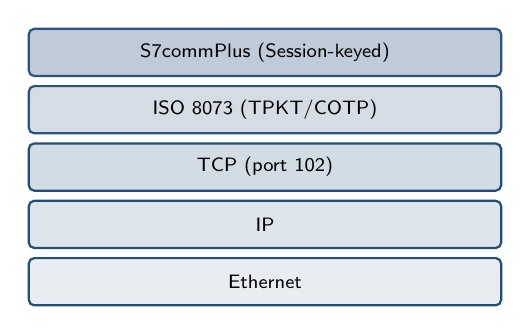
\begin{tikzpicture}[node distance=1mm]
  \node[isbox, fill=isOT!10, draw=isOT, minimum width=60mm, minimum height=6mm, font=\scriptsize] (eth) {Ethernet};
  \node[isbox, fill=isOT!15, draw=isOT, minimum width=60mm, minimum height=6mm, font=\scriptsize, above=of eth] (ip) {IP};
  \node[isbox, fill=isOT!20, draw=isOT, minimum width=60mm, minimum height=6mm, font=\scriptsize, above=of ip] (tcp) {TCP (port 102)};
  \node[isbox, fill=isPLC!20, draw=isPLC, minimum width=60mm, minimum height=6mm, font=\scriptsize, above=of tcp] (cotp) {ISO 8073 (TPKT/COTP)};
  \node[isbox, fill=isPLC!30, draw=isPLC, minimum width=60mm, minimum height=6mm, font=\scriptsize, above=of cotp] (s7p) {S7commPlus (Session-keyed)};
\end{tikzpicture}
\vspace{2mm}
\begin{importantbox}{Session keys, not real crypto}
Each session derives a key from challenges in the handshake -- but the key derivation function (KDF) is fixed and reproducible. Several research groups have re-implemented it.
\end{importantbox}
\source{Biham, E., Bitan, S., Carmel-Veilleux, A., et al., \emph{Rogue7: Rogue Engineering-Station Attacks on S7 Simatic}, Black Hat USA, 2019.}
\end{frame}

\begin{frame}[fragile]{S7commPlus Frame Sketch}
\centering
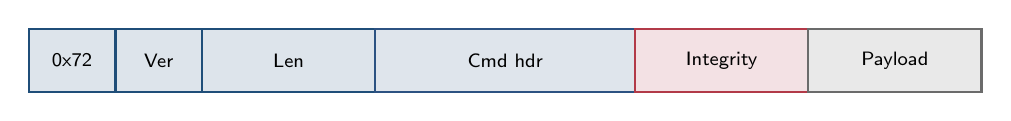
\begin{tikzpicture}[x=11mm, y=8mm, font=\scriptsize]
  \foreach \x/\w/\name/\col in {0/1/{0x72}/isOT, 1/1/{Ver}/isOT, 2/2/{Len}/isOT, 4/3/{Cmd hdr}/isPLC, 7/2/{Integrity}/isAttack, 9/2/{Payload}/isMute}{
    \draw[fill=\col!15, draw=\col, thick] (\x,0) rectangle ++(\w,1);
    \node[align=center] at (\x+\w/2, 0.5) {\name};
  }
\end{tikzpicture}
\vspace{2mm}
\begin{notebox}{Open-source dissectors}
\texttt{python-s7commplus} (gymgle, 2018) and \texttt{Plc4j} / \texttt{Plc4go} (Apache) both implement S7commPlus enough to read tags. Wireshark has a partial dissector.
\end{notebox}
\source{Lei, C.\ et al., \emph{S7commPlus reverse engineering}, 2017--2020 \textbar{} Wireshark \texttt{s7comm-plus} dissector (\texttt{epan/dissectors/packet-s7comm-plus.c}).}
\end{frame}

\section{IEC 61850 Stack}

\begin{frame}{IEC 61850 -- The Substation Stack}
\centering
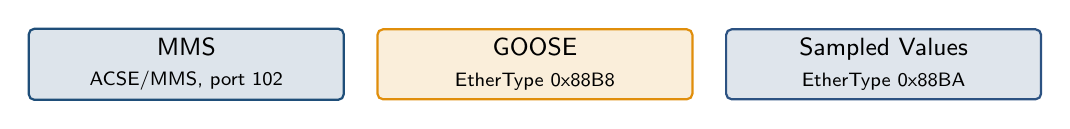
\begin{tikzpicture}[node distance=4mm]
  \node[isbox, fill=isOT!15, draw=isOT, minimum width=40mm, font=\small] (mms) {MMS\\\scriptsize ACSE/MMS, port 102};
  \node[isbox, fill=isAccent!15, draw=isAccent, minimum width=40mm, font=\small, right=of mms] (gse) {GOOSE\\\scriptsize EtherType 0x88B8};
  \node[isbox, fill=isPLC!15, draw=isPLC, minimum width=40mm, font=\small, right=of gse] (sv) {Sampled Values\\\scriptsize EtherType 0x88BA};
\end{tikzpicture}
\vspace{2mm}
\begin{importantbox}{GOOSE has no authentication by default}
Multicast L2 frames, 3\,ms total transfer time (IEC 61850-5 type 1A trip), sequence-number anti-replay only. IEC 62351 adds signatures but adoption in production substations is rare.
\end{importantbox}
\source{IEC 61850 (multipart) \textbar{} IEC 62351 (security for TC 57 protocols).}
\end{frame}

\begin{frame}{GOOSE Frame Anatomy}
\centering
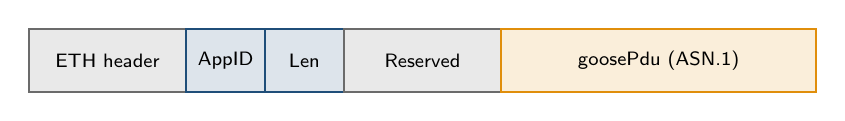
\begin{tikzpicture}[x=10mm, y=8mm, font=\scriptsize]
  \foreach \x/\w/\name/\col in {0/2/{ETH header}/isMute, 2/1/{AppID}/isOT, 3/1/{Len}/isOT, 4/2/{Reserved}/isMute, 6/4/{goosePdu (ASN.1)}/isAccent}{
    \draw[fill=\col!15, draw=\col, thick] (\x,0) rectangle ++(\w,1);
    \node[align=center] at (\x+\w/2, 0.5) {\name};
  }
\end{tikzpicture}
\vspace{2mm}
\begin{notebox}{Known weakness}
A spoofed GOOSE with a higher \texttt{stNum} (status number) is accepted instantly. Without IEC 62351-6, the only mitigation is L2 isolation.
\end{notebox}
\source{C.\ Kush, A.\ Ahmadian, P.\ Mahgoub, et al., academic GOOSE attack papers 2010--2018.}
\end{frame}

\section{MMS \& DLMS/COSEM}

\begin{frame}{MMS -- Manufacturing Message Specification}
\begin{itemize}
  \item Application-layer ISO 9506, runs over OSI on TCP/IP (RFC 1006).
  \item Identifies named variables and methods on an IED.
  \item Used by IEC 61850 for client-server (HMI talks to IED here).
  \item No authentication by default; IEC 62351 part 4 adds TLS for MMS.
\end{itemize}
\begin{notebox}{Why MMS matters}
The HMI's read/write of named variables flows through MMS. If you can spoof or replay MMS, you can drive the IED's behaviour from the operator's perspective.
\end{notebox}
\source{ISO 9506 (Parts 1 and 2) \textbar{} IEC 62351-4.}
\end{frame}

\begin{frame}{DLMS/COSEM -- Smart Meters}
\centering
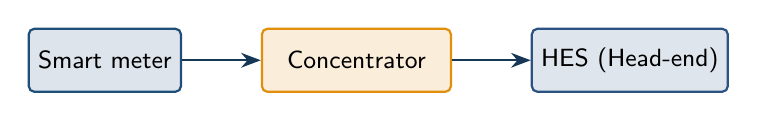
\begin{tikzpicture}[node distance=10mm]
  \node[isbox, fill=isOT!15, draw=isOT, font=\small] (m) {Smart meter};
  \node[isbox, fill=isAccent!15, draw=isAccent, right=of m, font=\small, minimum width=24mm] (con) {Concentrator};
  \node[isbox, fill=isPLC!15, draw=isPLC, right=of con, font=\small, minimum width=24mm] (hes) {HES (Head-end)};
  \foreach \s/\e in {m/con, con/hes}{\draw[flow] (\s) -- (\e);}
\end{tikzpicture}
\vspace{2mm}
\begin{notebox}{Authentication levels}
DLMS defines mechanism IDs 0--7 (IEC 62056-5-3): 0 = none, 1 = LLS (shared password), 2--7 = HLS variants (MD5, SHA-1, GMAC, SHA-256, ECDSA). German rollout (BSI TR-03109) mandates Gateway with X.509 + AES-GCM.
\end{notebox}
\source{IEC 62056 (DLMS/COSEM Blue/Green/Yellow/White books) \textbar{} BSI TR-03109.}
\end{frame}

\section{Building Dissectors and Fuzzers}

\begin{frame}[fragile]{Custom Scapy Layer (sketch)}
\begin{lstlisting}[language=Python]
from scapy.all import Packet, ByteField, ShortField, bind_layers, TCP

class MyVendor(Packet):
    name = "MyVendor"
    fields_desc = [
        ByteField("magic", 0x5A),
        ByteField("version", 1),
        ShortField("length", None),
    ]

bind_layers(TCP, MyVendor, sport=27015)
bind_layers(TCP, MyVendor, dport=27015)
\end{lstlisting}
\vspace{2mm}
\begin{tipbox}{First step}
Capture a known-good session, hex-edit one byte at a time, replay -- watch the device's reaction. That tells you which fields gate what.
\end{tipbox}
\source{P.\ Biondi et al., \emph{Scapy} project documentation, \url{https://scapy.readthedocs.io} \textbar{} Scapy contrib ICS modules (Modbus, ENIP/CIP).}
\end{frame}

\begin{frame}{Fuzzing ICS Protocols}
\centering
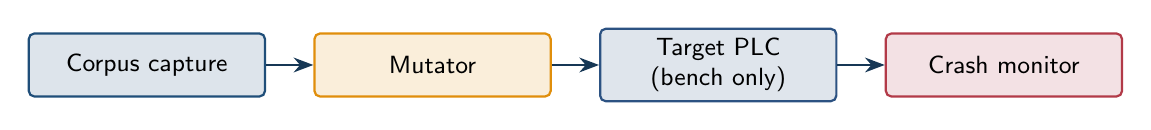
\begin{tikzpicture}[node distance=6mm]
  \node[isbox, fill=isOT!15, draw=isOT, minimum width=30mm, font=\small] (corp) {Corpus capture};
  \node[isbox, fill=isAccent!15, draw=isAccent, right=of corp, minimum width=30mm, font=\small] (mut) {Mutator};
  \node[isbox, fill=isPLC!15, draw=isPLC, right=of mut, minimum width=30mm, font=\small] (tgt) {Target PLC\\(bench only)};
  \node[isbox, fill=isAttack!15, draw=isAttack, right=of tgt, minimum width=30mm, font=\small] (mon) {Crash monitor};
  \draw[flow] (corp) -- (mut); \draw[flow] (mut) -- (tgt); \draw[flow] (tgt) -- (mon);
\end{tikzpicture}
\vspace{2mm}
\begin{warnbox}{Bench only}
Industrial devices crash on malformed input -- often by tripping the safety system. \emph{Never} fuzz production. Use a spare unit on a private VLAN.
\end{warnbox}
\source{Tools: \texttt{boofuzz}, \texttt{kitty}/\texttt{katnip}, AFL++ for TCP harnesses.}
\end{frame}

\begin{frame}{Implementation Defects to Watch}
\begin{itemize}
  \item Integer overflows in length fields (Ripple20, URGENT/11, NUCLEUS:13).
  \item Out-of-bounds writes in ASN.1 parsers (MMS, GOOSE).
  \item Reproducible session-key derivation in challenge-response auth (Rogue7, 2019).
  \item Hard-coded session keys after firmware update (multiple vendors).
  \item ICS PSIRT disclosures often reveal these for one product but the same code is in twenty others.
\end{itemize}
\source{Forescout Vedere Labs, \emph{Project Memoria}: Ripple20, URGENT/11, NUCLEUS:13, NAME:WRECK, INFRA:HALT.}
\end{frame}

\section{Defensive View}

\begin{frame}{What an ICS IDS Can / Cannot See}
\centering
\renewcommand{\arraystretch}{1.3}
\footnotesize
\setlength{\tabcolsep}{3pt}
\begin{tabular}{|p{3.4cm}|p{4.4cm}|p{4.4cm}|}
\hline
\rowcolor{slidePanel}
\textbf{Protocol} & \textbf{Detectable} & \textbf{Hidden} \\
\hline
Modbus TCP   & function code, addr, value & nothing -- plain \\
S7commPlus   & frame, command ID          & encrypted payload \\
GOOSE        & ETH header, AppID, stNum   & multicast L2 only \\
DLMS/COSEM   & AARQ, COSEM class IDs      & encrypted, depending on level \\
\hline
\end{tabular}
\vspace{2mm}
\begin{notebox}{Implication}
Span-port IDS gives full visibility on legacy plaintext stacks and only partial visibility on session-keyed stacks. Plan host telemetry for the latter.
\end{notebox}
\source{Zeek Project, \emph{Zeek Network Monitor}, \url{https://zeek.org} \textbar{} CISA \texttt{cisagov/icsnpp} ICS protocol parsers \textbar{} MITRE ATT\&CK for ICS (v14, 2024).}
\end{frame}

%% Frame 1: IEC 62351 / 62443-3-3 standards anchor
\begin{frame}{Security-standard anchor for advanced protocols}
\centering
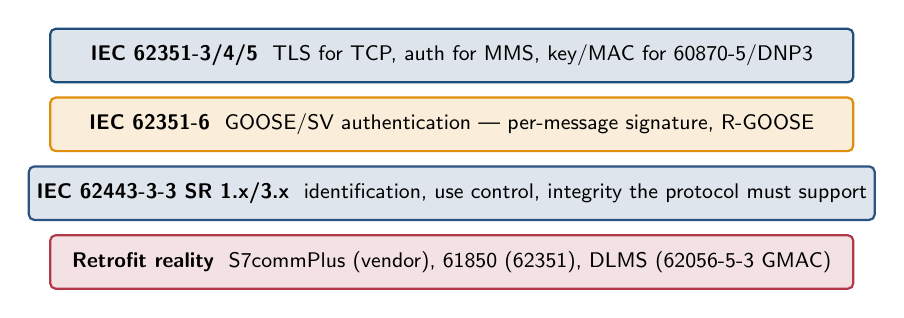
\begin{tikzpicture}[node distance=2mm, scale=0.85, transform shape]
  \node[isbox, fill=isOT!15, draw=isOT, minimum width=120mm, font=\small] (a)
    {\textbf{IEC 62351-3/4/5} \ TLS for TCP, auth for MMS, key/MAC for 60870-5/DNP3};
  \node[isbox, fill=isAccent!15, draw=isAccent, minimum width=120mm, font=\small, below=of a] (b)
    {\textbf{IEC 62351-6} \ GOOSE/SV authentication --- per-message signature, R-GOOSE};
  \node[isbox, fill=isPLC!15, draw=isPLC, minimum width=120mm, font=\small, below=of b] (c)
    {\textbf{IEC 62443-3-3 SR 1.x/3.x} \ identification, use control, integrity the protocol must support};
  \node[isbox, fill=isAttack!15, draw=isAttack, minimum width=120mm, font=\small, below=of c] (d)
    {\textbf{Retrofit reality} \ S7commPlus (vendor), 61850 (62351), DLMS (62056-5-3 GMAC)};
\end{tikzpicture}
\par\vspace{2mm}
{\footnotesize 62351 is the bolt-on crypto layer for the TC~57 protocols; 62443-3-3 fixes \emph{which} system requirements (SR) the deployed protocol must meet at each security level.}
\source{IEC 62351 (multipart) \textbar{} IEC 62443-3-3:2013 SR\,1--7 \textbar{} IEC 62056-5-3.}
\note{
  This is the spine for the whole section. 62351 retrofits crypto onto protocols designed in the 1990s with zero security; 62443-3-3 is the system-level checklist of foundational requirements (FR1 identification \& authentication, FR3 system integrity, FR4 data confidentiality) that the deployed protocol must satisfy at SL 1--4. Make the split explicit: 62351 is the mechanism, 62443-3-3 is the requirement that drives whether you must turn it on. Stress that adoption lags badly --- most substations and meters run the plaintext base protocol because the retrofit costs latency and key management. S7commPlus is the odd one out: vendor-proprietary crypto, no 62351 coverage. Transition: ``Start with the one that pretends to be secure --- S7commPlus.''
}
\end{frame}

%% Frame 2: S7commPlus anti-replay internals
\begin{frame}[fragile]{S7commPlus anti-replay --- challenge/response internals}
\centering
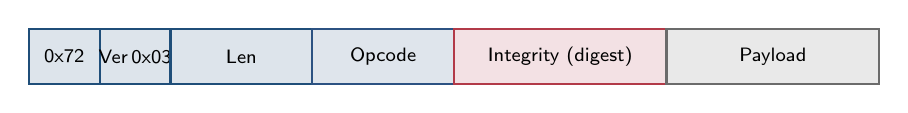
\begin{tikzpicture}[x=9mm, y=7mm, font=\scriptsize]
  \foreach \x/\w/\name/\col in {0/1/{0x72}/isOT, 1/1/{Ver\,0x03}/isOT, 2/2/{Len}/isOT, 4/2/{Opcode}/isPLC, 6/3/{Integrity (digest)}/isAttack, 9/3/{Payload}/isMute}{
    \draw[fill=\col!15, draw=\col, thick] (\x,0) rectangle ++(\w,1);
    \node[align=center] at (\x+\w/2, 0.5) {\name};
  }
\end{tikzpicture}
\par\vspace{0.5mm}
{\footnotesize The \emph{integrity} field is a keyed digest over opcode + payload --- the per-session anti-replay/anti-tamper guard.}
\par\vspace{0.5mm}
\begin{importantbox}{Why early versions were defeated}
The handshake digest (\texttt{0x011d}/\texttt{0x011e}) derives a session key from a server \emph{challenge}, but the KDF and seed constants are baked into the firmware --- so the per-session integrity field is \emph{recomputable offline}. Capture one challenge, replay with a valid digest.
\end{importantbox}
\begin{notebox}{Hardening (v3 protocol, S7-1500 FW $\geq$ 2.x)}
Later firmware adds a non-derivable nonce and binds the digest to TLS transport --- the offline-recompute path closes; legacy units in compatibility mode stay exposed.
\end{notebox}
\source{Lei, C.\ et al., \emph{S7commPlus reverse engineering}, 2017--2020 \textbar{} Cheng, L., \emph{Wireshark s7comm-plus dissector notes}.}
\note{
  This is the depth jump from the Bachelor view. The earlier frame in this deck says ``session keying is reproducible'' --- here we say exactly why. The integrity field is a keyed digest over opcode+payload, intended as anti-replay/anti-tamper. The defeat is not a crypto break: the KDF inputs (challenge) are observable on the wire and the KDF constants are static in firmware, so an attacker reconstructs the same key the PLC will. Emphasise the difference between obfuscation and authentication: a key both endpoints can derive from public data authenticates nobody. The byte sketch is deliberately simplified --- real frames carry TLV item lists --- but the integrity field's position relative to opcode/payload is the load-bearing detail. Mitigation only lands when the digest is bound to a transport secret the attacker cannot derive. Transition: ``S7commPlus at least tries; GOOSE ships sub-4ms frames with a sequence counter and nothing else.''
}
\end{frame}

%% Frame 3: IEC 61850 GOOSE/SV timing & spoofing
\begin{frame}{GOOSE/SV timing window and the spoofing race}
\centering
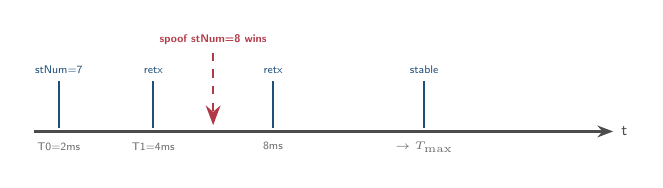
\begin{tikzpicture}[font=\scriptsize, node distance=0mm, scale=0.8, transform shape]
  \draw[axisline] (0,0) -- (9.2,0) node[right] {t};
  \foreach \x/\lbl/\dt in {0.4/{stNum=7}/T0=2ms, 1.9/{retx}/T1=4ms, 3.8/{retx}/8ms, 6.2/{stable}/$\to T_{\max}$}{
    \draw[isOT, thick] (\x,0.05) -- (\x,0.8);
    \node[isOT, font=\tiny, anchor=south] at (\x,0.8) {\lbl};
    \node[isMute, font=\tiny, anchor=north] at (\x,-0.05) {\dt};
  }
  \draw[attack] (2.85,1.25) -- (2.85,0.1);
  \node[isAttack, font=\tiny\bfseries, anchor=south] at (2.85,1.25)
    {spoof stNum=8 wins};
\end{tikzpicture}
\par\vspace{1mm}
\begin{importantbox}{The spoofing window}
Each event triggers a burst of retransmissions (\texttt{stNum}++, \texttt{sqNum}=0). A forged frame with a \emph{higher} \texttt{stNum} is trusted instantly --- no origin check, no time to react inside the 3ms trip budget.
\end{importantbox}
\begin{notebox}{Mitigation: IEC 62351-6 / R-GOOSE}
Per-message signing (R-GOOSE over UDP/IP) authenticates the publisher and seals \texttt{stNum}/\texttt{sqNum}; verify latency must still fit the 3ms P1 budget --- HW MAC, not RSA.
\end{notebox}
\source{IEC 61850-8-1 / IEC 61850-90-5 (R-GOOSE) \textbar{} IEC 62351-6:2020.}
\note{
  Master-level GOOSE: the Bachelor view stopped at ``higher stNum is accepted.'' Here we make the timing concrete. stNum increments on every state change and resets sqNum to 0; between events sqNum just counts retransmissions. The publisher floods retransmits at shrinking intervals (T0~2ms growing toward a stable ~16ms-1s heartbeat). The attacker only needs to inject one frame with stNum greater than the legitimate counter during that burst --- the subscriber accepts the newest state with no source authentication. Tie the impossibility of naive defence to the timing class: trip messages are performance class P1, 3ms transfer time, so you cannot afford asymmetric crypto on the verify path. That is why 62351-6 specifies a MAC/signature scheme amenable to hardware acceleration, and why R-GOOSE matters when the message must leave the L2 segment. Ask students: what does signing buy you if the key is shared substation-wide? (Answer: integrity, not non-repudiation --- segue to key management.) Transition: ``Same key-management problem at scale --- millions of meters running DLMS/COSEM.''
}
\end{frame}

%% Frame 4: DLMS/COSEM & smart-metering security
\begin{frame}{DLMS/COSEM --- association, HLS-GMAC, key hierarchy}
\centering
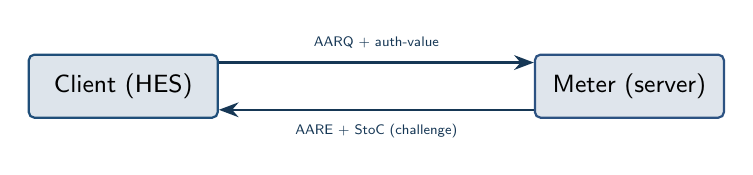
\begin{tikzpicture}[node distance=7mm, font=\scriptsize]
  \node[isbox, fill=isOT!15, draw=isOT, minimum width=24mm] (c) {Client (HES)};
  \node[isbox, fill=isPLC!15, draw=isPLC, minimum width=24mm, right=40mm of c] (m) {Meter (server)};
  \draw[flow] ([yshift=3mm]c.east) -- node[above, font=\tiny, yshift=0.5mm] {AARQ + auth-value} ([yshift=3mm]m.west);
  \draw[flow] ([yshift=-3mm]m.west) -- node[below, font=\tiny, yshift=-0.5mm] {AARE + StoC (challenge)} ([yshift=-3mm]c.east);
\end{tikzpicture}
\par\vspace{1.5mm}
{\footnotesize Key hierarchy: \textbf{Master Key} (KEK) wraps $\rightarrow$ \textbf{AK} (authentication, HLS-GMAC) and \textbf{EK} (encryption, AES-128-GCM), each per-association.}
\par\vspace{1.5mm}
\begin{notebox}{Metering attack surface}
HLS level 5 (GMAC): forged StoC/CtoS or nonce reuse breaks the GCM auth; a leaked global broadcast EK (firmware extraction) decrypts whole concentrator segments. Low-Level Security (shared password) and security-suite-0 fallbacks remain the practical entry. BSI TR-03109 forces the gateway to terminate this in tamper-resistant HW.
\end{notebox}
\source{IEC 62056-5-3 (DLMS green book) \textbar{} IEC 62056-6-2 security suites \textbar{} BSI TR-03109-1.}
\note{
  Deepens the Bachelor auth-level list into the actual mechanism. The Application Association (AARQ/AARE) negotiates the authentication mechanism and exchanges the challenge for HLS; the auth-value carries the response. HLS-GMAC (mechanism 5) uses AES-GCM in MAC-only mode keyed by AK with a 12-byte IV = system-title || invocation-counter --- so invocation-counter monotonicity is security-critical; a reset or wrap enables nonce reuse and forgery. Walk the key hierarchy: a master/KEK wraps the per-association AK and EK; security suite 1 adds AES-GCM-128 for confidentiality. The brutal failure mode is the global broadcast key shared across a population --- one firmware extraction compromises a whole segment, exactly the systemic risk regulators fear. BSI TR-03109 answers this by mandating a Smart Meter Gateway with X.509 + secure element so keys never live in the cheap meter. Ask: why is the invocation counter the most attacked field? (Nonce reuse in GCM is catastrophic.) Close the section here.
}
\end{frame}


\begin{frame}{Summary -- Section \sectionNumber}
\begin{takeawaybox}{Advanced protocols, in one breath}
\begin{itemize}\setlength{\itemsep}{2pt}
  \item S7commPlus session keying is reproducible -- treat it as obfuscation, not crypto.
  \item GOOSE has no authentication by default; IEC 62351 changes this but adoption is rare.
  \item MMS and DLMS/COSEM both bolted security on later; rollouts have known weak modes.
  \item Custom dissectors (Scapy, Wireshark) unlock visibility on niche vendor protocols.
  \item Fuzz only on bench equipment -- production devices crash unsafely.
\end{itemize}
\end{takeawaybox}
\end{frame}

\referencesframe{
  \item \emph{Cross-reference (prerequisites):} Bachelor \S\,04 (\emph{Protocols}) introduces Modbus, S7, OPC UA and IEC 61850 at the basic level; this section pushes into security internals.
  \item IEC 61850 (multipart). \emph{Communication networks and systems for power utility automation}.
  \item IEC 62351 (multipart), incl.\ IEC 62351-6:2020. \emph{Security for IEC TC 57 protocols}.
  \item ISO 9506. \emph{Manufacturing Message Specification (MMS)}, Parts 1 \& 2.
  \item IEC 62056. \emph{DLMS/COSEM} (Blue/Green/Yellow/White books).
  \item BSI TR-03109. \emph{Smart Metering System Specifications}.
  \item Beresford, D. \emph{Exploiting Siemens Simatic S7 PLCs}, BlackHat USA, 2011.
  \item Gordeychik, S. \emph{SCADA StrangeLove} talks and tools, 2014--2018.
  \item Lei, C.\ et al. Reverse-engineering of S7commPlus, academic papers, 2017--2020.
  \item Forescout Vedere Labs. \emph{Project Memoria} -- Ripple20, URGENT/11, NUCLEUS:13, NAME:WRECK, INFRA:HALT.
  \item Wireshark Foundation. ICS protocol dissectors (incl.\ \texttt{packet-s7comm-plus.c}).
  \item Biondi, P.\ et al. \emph{Scapy}, \url{https://scapy.readthedocs.io}; ICS contrib modules.
  \item \texttt{boofuzz} project (Joshua Pereyda). \url{https://boofuzz.readthedocs.io}.
  \item Apache Software Foundation. \emph{Plc4x} (Plc4j, Plc4go, Plc4py).
  \item Zeek Project. \emph{Zeek Network Monitor}, \url{https://zeek.org}.
  \item CISA. \texttt{cisagov/icsnpp} -- ICS Network Protocol Parsers for Zeek.
  \item MITRE. \emph{ATT\&CK for ICS}, v14, 2024.
}

\closingframe

\end{document}
